\section{Datenbeschreibung}
\label{sec:Datenbeschreibung}

Der vorliegende Datensatz besteht aus insgesamt 949 Bildern von Autos mit
Nummernschildern.\footnote{Die Originaldaten sind unter \url{https://github.com/phibuc/Lab_FS_Data},
    sowie unter \url{https://github.com/RobertLucian/license-plate-dataset}
    einsehbar.}
Die Bilder wurden in den Regionen Brasilien, Europa, Rum\"anien und USA
aufgenommen.

Zu jedem dieser Bilder liegen sowohl Informationen zur Position
des Nummernschildes innerhalb des Bildes, als auch zum
Inhalt des Nummernschildes vor.
Die Position des Nummernschildes ist dabei durch die Angabe von Pixel Koordinaten
$x_{\text{min}}$, $x_{\text{max}}$, $y_{\text{min}}$, $y_{\text{max}}$
relativ zur linken oberen Ecke des Bildes eindeutig spezifiziert.
In Abbildung~\ref{fig:autos} sind drei Beispielbilder aus dem Datensatz
dargestellt. Die Koordinaten der Nummernschilder sind anhand der
roten Rechtecke eingezeichnet.

Zur weiteren Verarbeitung der Bilder werden diese von nun an als Matrizen
aufgefasst, deren Eintr\"age genau den Pixeln im Bild zuzuordnen sind.
Da es sich hier um Farbaufnahmen handelt, ben\"otigt man f\"ur jedes
Bild sogar drei Matrizen, eine f\"ur jeden der drei Farbkan\"ale
Rot, Gr\"un und Blau (RGB).
Beispielsweise kann ein Bild mit einer Aufl\"osung von 100x100 Pixeln also
als Element des $\mathbb{R}^{100 \times 100 \times 3}$ beschrieben werden.
Solche \glqq dreidimensionalen Matrizen\grqq{} werden in der
Fachsprache auch als
\textbf{Tensoren}~\cite{Goodfellow-et-al-2016} bezeichnet.


\begin{figure}
    \centering
    \begin{subfigure}{0.32\textwidth}
        \centering
        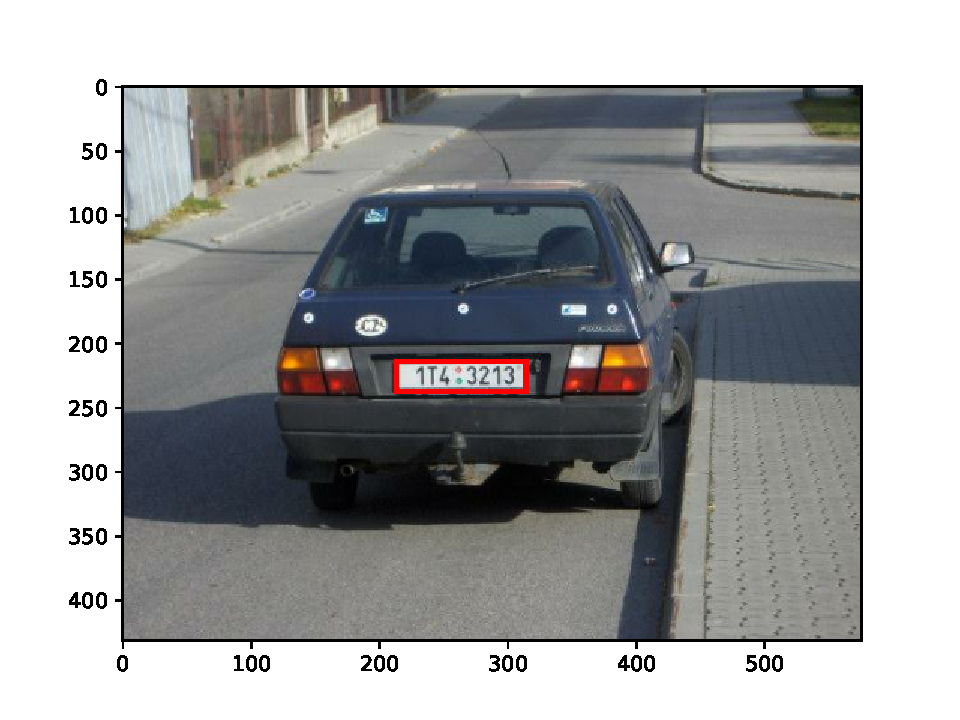
\includegraphics[width=\textwidth]{abbildungen/car_1}
    \end{subfigure}
    \begin{subfigure}{0.32\textwidth}
        \centering
        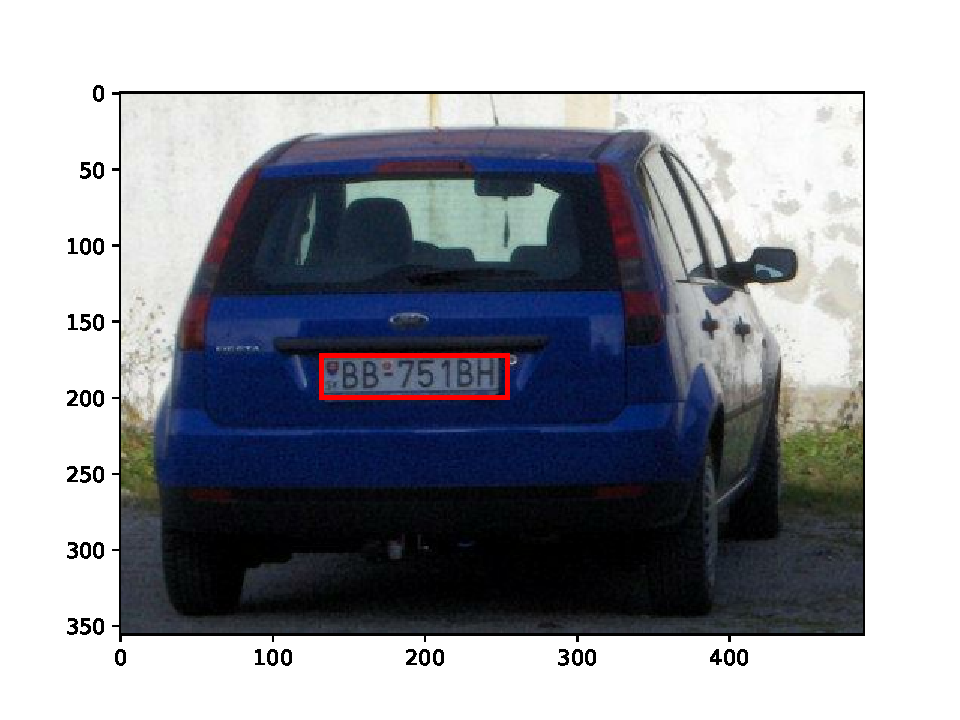
\includegraphics[width=\textwidth]{abbildungen/car_2}
    \end{subfigure}
    \begin{subfigure}{0.32\textwidth}
        \centering
        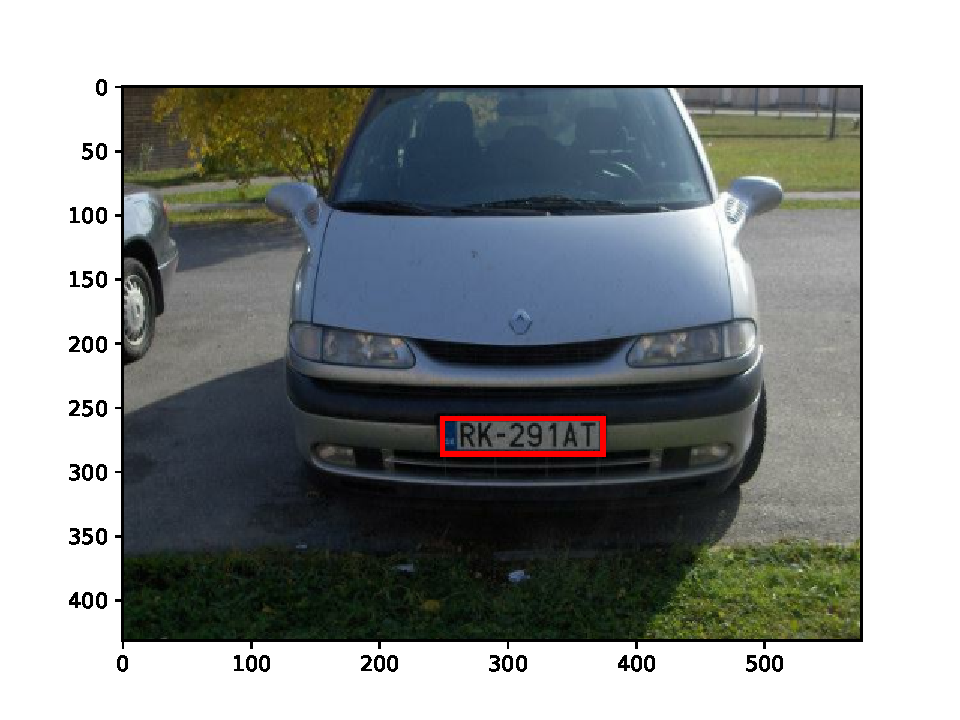
\includegraphics[width=\textwidth]{abbildungen/car_3}
    \end{subfigure}
    \caption[Beispielbilder]{Drei Beispiele aus dem vorliegenden Datensatz.
        Die Nummernschilder sind anhand ihrer Koordinaten rot umrandet.}
    \label{fig:autos}
\end{figure}